\documentclass[12pt]{article}

% Language setting
\usepackage[utf8]{inputenc}
\usepackage[bulgarian]{babel}

% --------------------- Packages  --------------------
% Use biblatex
\usepackage{biblatex}
\addbibresource{bibliography.bib}

% Include graphics
\usepackage{graphicx}
 
% Updated definition
% \newcommand*{\fullref}[1]{\ref*{#1}. \nameref*{#1}} % One single link
\newcommand*{\fullref}[1]{\ref*{#1}} % One single link

% --------------------- Title  --------------------
\title{Стробоскопичен метод за изследване на механични движения}
\author{Виолета Кабаджова}
\date{October 2022}

\begin{document}

% Anfang der Titelseite________________________________________________________________________________
\begin{titlepage}
	\flushleft
% 	\begin{center}
	%{\scshape\Large Werkstoffe III \hspace{2.5cm} Laborbericht \hspace{2.5cm}HS 2022 \par}
	{\scshape\Large Протокол II \hspace{2cm} Механика - практикум\par}
	\vspace{2cm}
	{\huge\bfseries Стробоскопичен метод за измерване на механични движения\par}
	\vspace{1cm}
	{\LARGE\bfseries Лабораторно упражнение №2\par}
	\vspace{6cm}
    % {\LARGE\bfseries Физически Факлутет към Софийски Университет "Св. Климент Охридски"\par}
    {\LARGE\bfseries Виолета Кабаджова, \par}
%   {\LARGE\bfseries Group: X\par}
    {\large\bfseries ККТФ, факл. номер: 3PH0600026\par}
	\vspace{1cm}
	
	{\large Физически Факлутет, 
	
	Софийски Университет "Св. Климент Охридски",
	
	03 ноември 2022 г.\par}
	
\end{titlepage}
\section{Теоритична част}

\begin{figure}
\centering
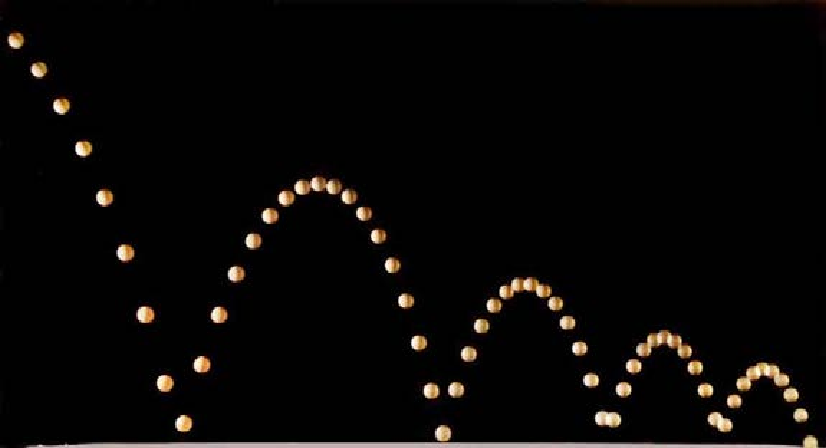
\includegraphics[width=1\textwidth]{images/stroboscopic-img-basic.png}
\caption{\label{fig:strob-img-basic} Стробоскопична картина на отскачаща топка. Ресурс: ResearchGate \cite{Driscoll2016}.}
\end{figure}

Стробоскопичният метод позволява определяне положението на движещо се тяло при равномерни и достатъчно малки интервали от време \(\tau\). При този метод движението на дадено тяло се регистрира върху хартия или на снимка, което позволява измерването кинематични величини, определянето на закона за движение, както и силите, които предизвикват това движение. За целта стробоскопичната снимка е необходимо да включва и подходящо разположени еталони за дължина, определящи нейния мащаб. На фиг. \ref{fig:strob-img-basic} е показана формата на една стробоскопична картина, макар и с липсващ мащаб на нея.

\subsection{Ограничение големината на интервалите}\label{sec:time-interval-limit}
Методът изисква ограничаване на големината на интервала от време \(\tau\), тъй като твърде голям интервал води до прекалено голяма грешка, и дори би могъл да пропусне крива от траекторията на тялото. Избирането на твърде малък интервал от своя страна би предизвикало резултатната снимка практически да наподобява непрекъсната линия, която описва единствено траекторията, но анализ на кинематичните величини при нея не би бил възможен поради незабелижимостта на разликите в разстоянията при участъците, през които тялото е преминало с по-голяма скорост, и тези, през които е преминало с по-малка.

\subsection{Методи за анализ на стробоскопична картина}

\begin{figure}
\centering
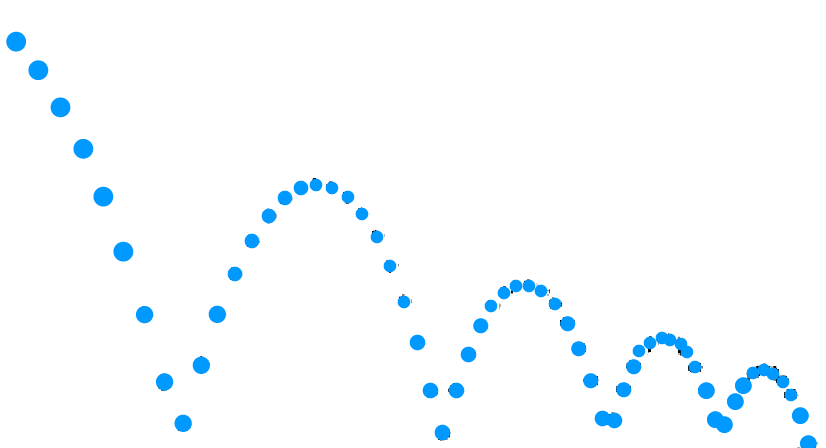
\includegraphics[width=1\textwidth]{images/stroboscopic-inv-img-blue.png}
\caption{\label{fig:strob-img-inverted} Стробоскопична картина на отскачаща топка от фиг. \ref{fig:strob-img-basic}, но улеснена за анализ.}
\end{figure}

Известни са два метода за анализ на стробоскопична картина - векторен и координатен.

\subsubsection{Векторен метод}
На фиг. \ref{fig:strob-img-inverted}, фиг. \ref{fig:strob-img-basic} е приведена във вид, по-удобен за работа. Нека \(\vec{r_1}\) и \(\vec{r_2}\) са радиус-векторите на две последователни премествания на материалната точка за два еднакви интервала от време \(\tau\). При позициониране на координатната си система така, че нейното начало да съвпада с началото на вектора \(\vec{r_1}\), тогава:

\begin{equation}\label{eq:delta-r}
\begin{aligned}
\Delta \vec{r_1} = \vec{r_1}, \\
\Delta \vec{r_2} = \vec{r_2} - \vec{r_1},
\end{aligned}
\end{equation}

Средните скорости в тези интервали са:

\begin{equation}\label{eq:delta-v}
\begin{aligned}
\vec{v_1} = \frac{\Delta \vec{r_1}}{t}, \\
\vec{v_2} = \frac{\Delta \vec{r_2}}{t}, \\
\end{aligned}
\end{equation}

Векторът \(\Delta \vec{v} = \vec{v_2} - \vec{v_1}\) е изменението на средната скорост за тялото между първия и втория интервал. Тогава от уравнение \ref{eq:delta-v} за средното ускорение \(\vec{a}\) се следва:

\begin{equation}\label{eq:a}
\vec{a} = \frac{\vec{v_2} - \vec{v_1}}{t} = \frac{1}{t^2}(\Delta \vec{r_2} - \Delta \vec{r_1})
\end{equation}

При  \(\tau\), клонящо към 0 ( \(\tau\)->0), средните стойностти на скоростта и ускорението ще клонят към съответните моментни скорости, но съгласно казаното в \fullref{sec:time-interval-limit} това не би могло да се определи по стробоскопичния метод поради невъзможността от коректно определяне на разстоянията между съответните положения.

\begin{figure}
\centering
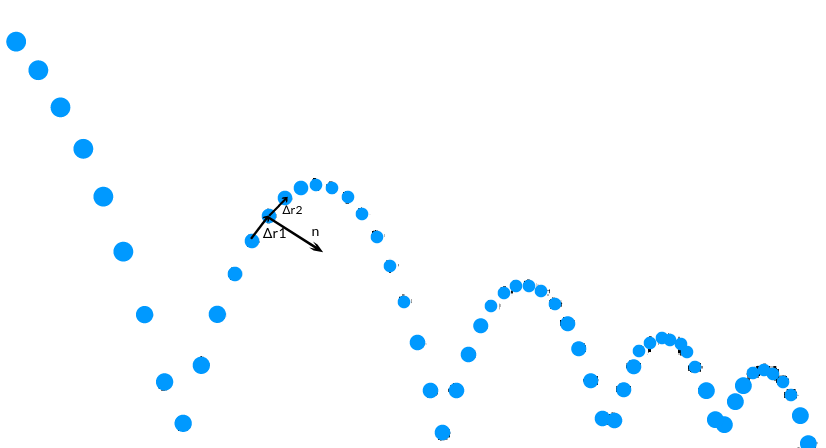
\includegraphics[width=1\textwidth]{images/vector-analysis.png}
\caption{\label{fig:vector-analysis} Разположение на вектори на преместване \(\Delta \vec{r_1}, \Delta \vec{r_2}\) и нормалата \(\vec{n}\)}
\end{figure}

На фиг. \ref{fig:vector-analysis} са показани вектори на преместване \(\Delta \vec{r_1}, \Delta \vec{r_2}\) и нормалата \(\vec{n}\). Големините на векторите на преместване \(\Delta \vec{r_i}\) са пропорционални на големините на средните скорости на тялото за съответните интервали: \(v_i = \frac{\Delta \vec{r_i}}{t}\), \([v_i] = m/s\). 

Разликата на два последователни вектора \(\Delta \vec{v} = \vec{v_{i+1}} - \vec{v_i}\) представлява изменението на средната скорост. Съгласно формула \ref{eq:a} \(\Delta \vec{v_i}\) е пропорционална на векрота на средното ускорение \(\vec{a}\), което е сума от тангенциално и нормално ускорение: \(\vec{a} = \vec{a_n} + \vec{a_\tau}\).

\subsubsection{Координатен метод}
Положението на материална точка спрямо отправна система може да се зададе и чрез нейните координати \((x(t), y(t), z(t))\). Тогава векторите \(\vec{r_1}\), \(\vec{r_2}\) са съответно с координати \((x_1, y_1\), \((x_2, y_2\). От начина на изменение на скоростта и ускорението, може да се определи вида на движението (дали е праволинейно или криволиейно). 

\begin{equation}\label{eq:v_coordinate_method}
v_{1x} = \frac{\Delta x_1}{t}, v_{1y} = \frac{\Delta y_1}{t},v_{2x} = \frac{\Delta x_2}{t}, v_{2y} = \frac{\Delta y_2}{t}
\end{equation}

\begin{equation}\label{eq:a_coordinate_method}
a_{x} = \frac{v_{2x} - v_{1x}}{t}, a_{y} = \frac{v_{2y} - v_{1y}}{t}
\end{equation}

Координатният метод е силно подходящ при изследване на праволинейни движения, но може да бъде използван и при криволинейни такива.

\subsubsection{Сила на триене}
Триенето бива три вида: сухо (между две твърди тела); вискозно (между течни или газообразни среди) и мокро (между твърдо тяло и течност или газ).

Съществуват три основни вида сухо триене: при покой, при хлъзгане и при търкаляне. Сухо триене при покой възниква, когато върху тялото се приложи външна сила. Тогава силата на триене е равна по големина и противоположна по посока на проекцията на приложената сила върху равнината, по която може да се хлъзга тялото. Поради това тялото остава в покой. В момента, в който големината на проекцията на приложената сила превиши определена критична стойност, тялото започва да се хлъзга, поради което силата на триене при хлъзгане бива приемана за максималната сила на триене при покой. Глемината на силата на триене не зависи т площта на триещите се повърхности и от големината на скоростта на двицение. Тя е пропорционална на нормалния натиск N, който тялото оказва върху равнината: \(F_тр = kN\), където k е коефициентът на триене при хлъзгане. При движение на тяло върхъ равнина, съгласно втория принцип на динамиката: 

\begin{equation}
F_x - F_{тр} = ma
\end{equation}


\section{Експериментална част}
\begin{figure}
\centering
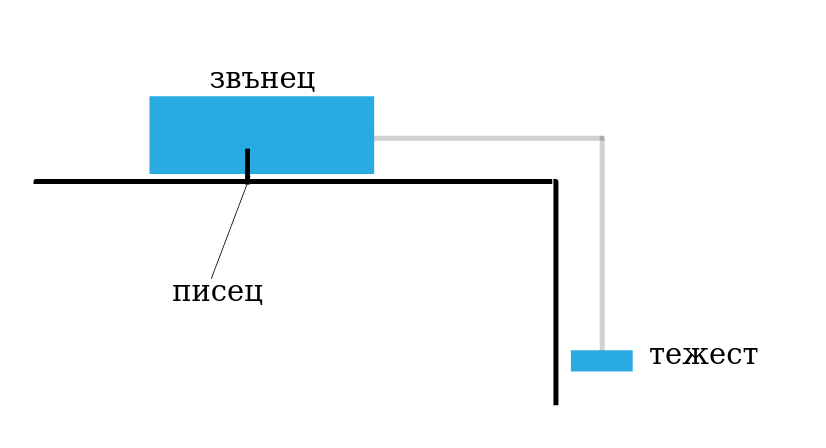
\includegraphics[width=1\textwidth]{images/bell_scheme.png}
\caption{\label{fig:linear-setup} Установка за съставяне на стробоскопична картина с праволинейна траектория.}
\end{figure}

\subsection{Експериментална установка}
За експеримента се използва звънец с честота 100 Hz. Оттук следва, че:

\begin{equation}
T = \frac{1}{\nu} = \frac{1}{100} = 0,01 s
\end{equation}

\subsubsection{Праволинейно движение}\label{sec:linear-movement}
За да получим стробоскопична картина, използваме звънец, за който е закрепен писец по такъв начин, че ударът на звънеца предизвиква писеца да удари повърхността под себе си. Слагайки лист хартия на повърхността с лист индиго над нея и закрепяйки за звънеца тежест, която да го придърпва чрез въженце, тялото извършва праволинейно движение. По този начин можем да отбележим скоростта на тялото, имайки неговата честота на звънене. Виж фиг. \ref{fig:linear-setup}.

\subsubsection{Криволинейно движнеие}
По подобен на начина, описан в \ref{sec:linear-movement}, можем да съставим и стробоскопична на криволинейно движение. Това се случва чрез взимане на звънеца и ръчното му придърване по произволна крива вместо използване на тежестта.

\subsection{Задачи}
\subsubsection{Задача 1: Определяне стойността на \(\vec{a}\) за два различни участъка от траекторията на праволинейно движение}

\begin{figure}
\centering
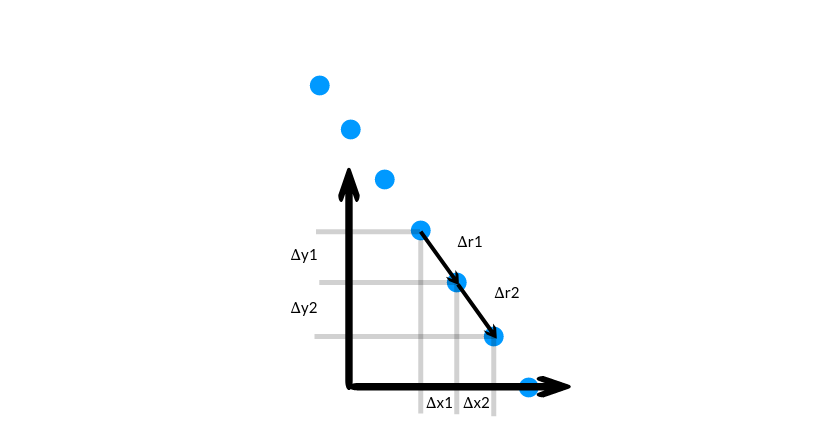
\includegraphics[width=1\textwidth]{images/linear-with-radius-vectors.png}
\caption{\label{fig:linear-with-radius-vectors} Праволинейно движение с два наложени радиус-вектора \(\Delta \vec{r_1}\) и \(\Delta \vec{r_2}\).}
\end{figure}

Използвайки опитната установка, описана в \ref{sec:linear-movement}, съставяме стробоскопична картина с праволинейна траектория. Тъй като движението е именно праволинейно, е удобно да използваме координатния метод за откриване на стойността на вектора на ускорението \(\vec{a}\). На фиг. \ref{fig:linear-with-radius-vectors} е показан модел, подобен на получения при провеждането на експеримента. Поради близостта на точките в реалната картина, взимаме точки, разположени през една с цел по-коректно измерване.

Измервайки разликите в две съседни положения в картината (две съседни положения наричаме положение през една точка), получаваме: \(\Delta x_1\) = 7 mm, \(\Delta x_2\) = 8 mm, \(\Delta y_1\) = 9 mm, \(\Delta y_2\) = 10 mm. Тогава от формули \ref{eq:v_coordinate_method}. следват следните стойности да скоростите по компоненти:

\begin{displaymath}
v_{1x} = \frac{\Delta x_1}{t} = \frac{7.10^{-3}}{2.10^{-2}} = 0,35 m/s, \\
\end{displaymath}

\begin{displaymath}
v_{1y} = \frac{\Delta y_1}{t} = \frac{9.10^{-3}}{2.10^{-2}} = 0,45 m/s,
\end{displaymath}

\begin{displaymath}
v_{2x} = \frac{\Delta x_2}{t} = \frac{8.10^{-3}}{2.10^{-2}} = 0,40 m/s,   
\end{displaymath}

\begin{displaymath}
v_{2y} = \frac{\Delta y_2}{t} = \frac{10.10^{-3}}{2.10^{-2}} = 0,50 m/s,    
\end{displaymath}

По формули \ref{eq:a_coordinate_method} следват следните стойности за ускорението по компоненти:

\begin{displaymath}
a_{x} = \frac{v_{2x} - v_{1x}}{t} = \frac{0,40 - 0,35}{0,02} = 2,5 m/s^2
\end{displaymath}

\begin{displaymath}
a_{y} = \frac{v_{2y} - v_{1y}}{t} = \frac{0,50 - 0,45}{0,02} = 2,5 m/s^2
\end{displaymath}


\subsubsection{Задача 2: Определяне на \(\vec{a_n}\) и \(\vec{a_\tau}\) при криволинейно движение за два участъка от траекторията с различен радиус на кривата}

\begin{figure}
\centering
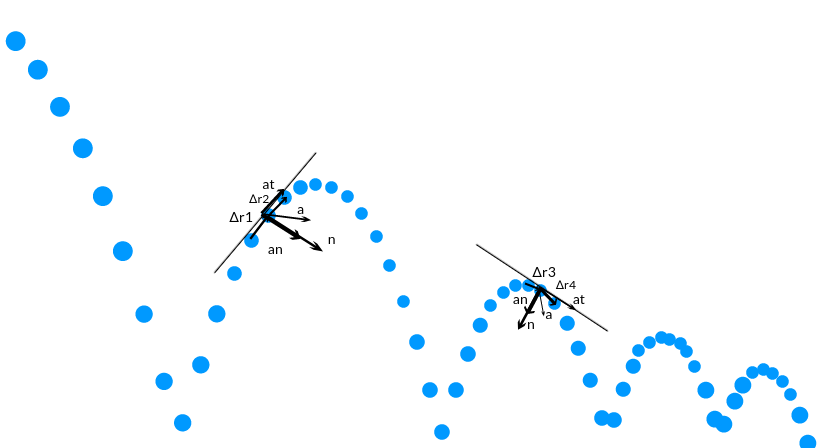
\includegraphics[width=1\textwidth]{images/circular_tangent_a.png}
\caption{\label{fig:circultar-tangent-a} Определяне на \(\vec{a_n}\) и \(\vec{a_\tau}\) за два различни участъка от траекторията.}
\end{figure}


Задачата се изпълнява графично на фиг. \ref{fig:circultar-tangent-a}. За целта взимаме две двойки вектори, всяка от които е в различна част от траекторията и във всяка двойка векторите са разположени между две съседни положения: \(\Delta \vec{r_1}\) и \(\Delta \vec{r_2}\), \(\Delta \vec{r_3}\) и \(\Delta \vec{r_4}\). Начертаваме нормалата, сочеща към центъра на окръжността, сформирана по кривата в конкретния момент, и започваща от края на втория вектор във всяка двойка (т.е. от върха на вектори \(\Delta \vec{r_1}\) и \(\Delta \vec{r_3}\)). По нея чертаем \(\vec{a_n}\) за всяка от двойките. \(\vec{a_\tau}\) лежи на допирателната към тази окръжност и е по посока на движението по траекторията. Сумата от тези два вектора сформира вектора на ускорението \(\vec{a}\).

От фигурата виждаме, че вектор \(\Delta \vec{r_1}\) е с по-голяма дължина от вектор \(\Delta \vec{r_2}\), откъдето заключваме, че движението в нея част от тректорията е закъснително. Аналогично установяваме, че \(||\Delta \vec{r_3}|| < ||\Delta \vec{r_4}||\), откъдето следва, че движението в частта от траекторията \(r_{34}\) е ускорително.
\pagebreak
\printbibliography

\end{document}